\clearpage
\setcounter{page}{1}
\maketitlesupplementary

\counterwithin{figure}{section}
\counterwithin{table}{section}
\counterwithin{equation}{section}
\renewcommand\thesection{\Alph{section}}
\renewcommand\thetable{\thesection.\arabic{table}}
\renewcommand\thefigure{\thesection.\arabic{figure}}
\renewcommand\theequation{\thesection.\arabic{equation}}
\setcounter{section}{0}

\renewcommand{\theHsection}{supp.\Alph{section}}
\renewcommand{\theHtable}{supp.\Alph{section}.\arabic{table}}
\renewcommand{\theHfigure}{supp.\Alph{section}.\arabic{figure}}
\renewcommand{\theHequation}{supp.\Alph{section}.\arabic{equation}}


This supplementary material is organized as follows:
\begin{itemize}
    \item \cref{sec:panshot} provides additional details on our construction of the camera-diverse dataset.
    \item \cref{sec:abs_orient} elaborates the derivation of the absolute orientation encoding.
    \item \cref{sec:eval} summarizes the evaluation metrics used in our experiments.
    \item \cref{sec:impl} presents implementation details for both our pipeline and the baselines.
    \item \cref{sec:limitation} discusses the robustness, generalization capability, limitations, and future work.
    \item \cref{sec:demo} includes a detailed demo video.
\end{itemize}



\section{Dataset Construction}
\label{sec:panshot}




The main paper introduced UCPE, a unified camera encoding that jointly models 6-DoF poses, intrinsics, and lens distortions.  
Training and evaluating such a representation in a camera-controllable video generation setting requires large-scale data with diverse motions, FoVs, and distortions.  
However, collecting such real-world data is extremely expensive due to the need for multiple lenses, hardware configurations, and extensive manual effort.

To overcome these limitations, we synthesize camera-diverse videos by using 360° panoramic footage as a flexible exploration space, from which videos can be projected into arbitrary virtual cameras.

We design a \emph{three-stage data synthesis pipeline} comprising:
(1) \emph{360° panoramic video curation} to extract high-quality, gravity-aligned exploration clips;
(2) \emph{realistic rotation emulation} by transferring camera motions from perspective videos with similar translations; and
(3) \emph{camera-diverse video synthesis} under varied intrinsics, distortions, and augmented rotations.  
While Sec.~4.1 of the main paper provides an overview, here we present the full details.

\subsection{Coordinate Conventions}
\label{sec:coord}

Throughout this supplementary material, we adopt a consistent 3D coordinate convention for all projection, ray-mapping, and pose-related computations.
The coordinate frame is defined as follows:
\begin{itemize}
    \item the \(x\)-axis points to the right of the image;
    \item the \(y\)-axis points downward (following image coordinates);
    \item the \(z\)-axis points forward, aligned with the viewing direction of the ERP camera.
\end{itemize}

Under this convention, the world-up direction is
\begin{equation}
\bm{u}^{\mathrm{wld}} = [0,\,-1,\,0]^\top,
\label{eq:world_up}
\end{equation}
which is used consistently across ERP projections, UCM ray mappings
(Sec.~\ref{sec:panshot}), and the construction of the Up map
(Sec.~\ref{sec:abs_orient}).

\subsection{360° Panoramic Video Curation}
\label{sec:panflow}


A key benefit of UCPE is controllability over absolute pitch and yaw, resolving the ambiguity in conventional camera-controlled T2V generation.  
This requires all training videos to share a gravity-aware world frame, which is difficult to obtain from in-the-wild footage.

Fortunately, many commercial 360° cameras produce stabilized, gravity-aligned equirectangular panoramas using calibrated lenses and onboard IMUs.
This ensures a consistent up vector, enabling virtual cameras defined inside the panoramic sphere to inherit absolute pitch and yaw.

We begin from the large-scale 4K resolution 360° video corpus of~\cite{wallingford2024image}, containing 24.1k YouTube videos with diverse scenes and motions.  
These raw videos contain issues such as scene cuts, watermarks, low-quality footage, non-equirectangular projections, or imperfect stabilization.
We therefore construct a multi-stage pipeline to filter low-quality clips and obtain high-quality gravity-aligned panoramas suitable for camera-diverse video synthesis.

\paragraph{Clip Segmentation.}
Video generation models require temporally consistent clips.  
We first apply a threshold-based transition detector~\cite{scenedetect2024} to remove hard cuts and black fades, but this method often misses subtle transitions (\eg, cross fades).  
We then run panoramic visual SLAM~\cite{sumikura2019openvslam} on each preliminary segment.  
Empirically, SLAM fails to track features across scene transitions, leading to ``tracking-lost'' signals.
By monitoring these signals, we split the preliminary clips into more refined segments with consistent scenes, which results in roughly 400k clips, each of 10 seconds.

\paragraph{Camera Pose and Rotation Score Extraction.}
We run second pass of SLAM in localization mode to obtain more accurate poses, yielding approximately 300k clips with valid estimates.
As discussed earlier, enabling absolute orientation supervision requires removing clips that are unstabilized or not gravity-aligned.  
Since stabilized 360° videos are typically gravity-consistent, we examine the rotational components of the estimated poses and discard clips exhibiting large drift.
To quantify this, we compute a rotation score defined as the maximum relative rotation between each frame and the first frame:
\begin{equation}
    \alpha_{\max}
    =
    \max_{i>0}
    \arccos\!\left(
        \frac{\mathrm{Tr}\!\left(\mathbf{R}_0^\top \mathbf{R}_i\right)-1}{2}
    \right),
\end{equation}
where $\mathbf{R}_0$ is the first-frame rotation and $\mathbf{R}_i$ denotes the rotation at frame $i$.
Clips with excessive drift are later removed in~\cref{sec:emulate_rot}, ensuring consistent gravity-aware orientations.

\paragraph{Quality Filtering.}
The raw 360° videos contain various artifacts, which we address using three complementary filtering strategies:
\begin{itemize}
    \item \textbf{Low-quality filtering:} We use Q-Align~\cite{wu2024q} to assess image quality, aesthetics, and video quality, and average these scores as a quality indicator for candidate selection in~\cref{sec:emulate_rot}.
    \item \textbf{Watermark filtering:} A watermark detector~\cite{watermark} is applied to each frame, and the averaged score is used as a watermark indicator for candidate selection.
    \item \textbf{vLLM-based filtering:} A custom vLLM-based filter~\cite{bai2025qwen2} (see~\cref{fig:filter}) identifies and removes clips that are non-equirectangular, low-quality, or contain overlays, missing edges, or other artifacts.
    The vLLM model also assigns each clip to most relevant POI (Point of Interest) categories~\cite{xia2025panowan} for later semantic balancing.
\end{itemize}


\paragraph{Trajectory Scale Normalization.}
Monocular SLAM recovers camera trajectories only up to an arbitrary scale, causing the same unit translation to appear faster in shallow scenes and slower in deeper ones.  
To ensure consistent motion across clips, we estimate a per-clip geometric scale and normalize all trajectories accordingly.
Specifically, we compute dense optical flow using PanoFlow~\cite{shi2023panoflow}, recover per-pixel depth via generalized epipolar geometry, and obtain a near-plane statistic by taking the 25th percentile of valid depths per frame and then the median across the clip.
We rescale each trajectory by this value so that the median near-plane depth becomes~1, yielding consistent apparent motion across all training clips.

\subsection{Emulating Realistic Camera Rotations}
\label{sec:emulate_rot}


The curated panoramic clips serve as exploration spaces with provided camera translations, but determining realistic camera rotations remains challenging.
Synthetic rotations (e.g., constant-speed sweeps) appear unnatural and do not reflect real panning, tilting, or rolling patterns that correlate with translation.

Our key insight is that videos with similar translation motions tend to exhibit similar rotation dynamics.
Thus, we employ a matching-based approach with two steps:
(1) extraction of realistic rotation trajectories from perspective videos, and
(2) matching and transferring these rotations to panoramic clips based on translation similarity and clip quality.


\paragraph{Candidate Rotation Extraction.}
We use CameraBench~\cite{lin2025towards}, a dataset of 1k motion-diverse cinematic videos with text-described camera motions.  
We remove clips with ``zoom'' in desciptions to maintain fixed intrinsics, and extract camera poses using ViPE~\cite{huang2025vipe}, producing around 300 unique trajectories.  
In some challenging scenarios, ViPE may produce unstable or jittery poses.
To remove these results, we compute each clip's maximum rotational velocity and discard the top 20\%.  
We then align all trajectories to a gravity-aware world frame via GeoCalib~\cite{veicht2024geocalib} by aligning the first-frame up vector to the world up axis.
This step ensures that all candidate rotations can be directly applied to the gravity-aligned panoramic clips to produce natural absolute orientations.

\paragraph{Trajectory Matching and Rotation Transfer.}
For each panoramic clip, we find CameraBench trajectories with similar translations and transfer their rotations to the virtual camera.
We first align each candidate trajectory to the panoramic clip via Umeyama fitting~\cite{umeyama2002least}, constrained to vertical-axis rotation.
Then we retain the top 30 candidates with lowest RMSE error for further selection.

The original 360° videos exhibit serious long tails in POI categories (see~\cref{fig:category_before}), possibly due to the widespread use of 360° cameras for specific scenarios such as outdoor sports in the mountains and street views.
Therefore we apply a series of diversity constraints during candidate selection to ensure semantic balance and motion diversity.
Specifically, each candidate is scored using a composite metric averaging quality score, watermark score, and the rotation score $\alpha_{\max}$ from~\cref{sec:panflow}.
Then they are traversed greedily from best to worst while enforcing the following diversity constraints:
\begin{itemize}
    \item \textbf{Panoramic clip diversity:} At most 5 CameraBench matches per panorama.
    \item \textbf{CameraBench trajectory diversity:} Each trajectory can be used at most 100 times.
    \item \textbf{POI semantic balance:} Matches are skipped if all POI categories of the panoramic clip already exceed 1000 matches.
    \item \textbf{Motion diversity:} We compute the average optical-flow magnitude as a motion score and maintain bins of fixed width of 10, each capped at 2000 samples.
\end{itemize}

While these constraints do not guarantee perfect uniformity, they substantially reduce long-tail distributions in POI categories (see~\cref{fig:category_after}) and motion.
After selection, each panoramic clip is paired with 5 per-frame camera rotations aligned to equirectangular coordinate system, yielding a total of 12k pairs of panoramic clips and rotation sequences.

\afterpage{
    \clearpage
    \begin{figure*}[t]
\centering
\begin{PromptBox}
You are a video understanding assistant specialized in analyzing panoramic ERP-format videos.  
Given one frame of a panoramic video, your tasks are:  

1. **Filtering**: Identify if the video should be filtered out.  
Output boolean flags for the following conditions (true if the issue exists, false otherwise):  

- non_ERP_format: The video is **not in ERP (Equirectangular Projection)** panoramic format. For example, if the video looks like a flat perspective, fisheye, cube-map, or any projection other than ERP, set this to true.  

- has_subtitle_or_watermark: The video contains **text overlays, subtitles, logos, or watermarks**. Look carefully for visible text at the bottom, center, or corners of the video. If such elements are present and not part of the real scene, set this to true.  

- edge_missing: The top or bottom edges of the ERP panorama are **cut off, blacked out, cropped, or covered by logos/watermarks**, so the full 360 vertical coverage is missing or obstructed. If you cannot clearly see the poles (sky/ground) or if the edges are hidden by overlays, set this to true.  

- has_overlay: The frame contains **artificial overlays**, such as embedded UI elements, pop-up graphics, stickers, video-in-video inserts, menus, or other synthetic elements that are not part of the natural scene. If you see signs of AR/VR interface, streaming UI, or added images, set this to true.  

- low_quality: The video is of **poor visual quality**, such as being blurry, noisy, heavily pixelated, very low resolution, or distorted in a way that prevents recognizing the scene. If the content is hard to interpret due to quality issues, set this to true.  

- unnatural_content: The video contains **cartoons, animations, CGI, synthetic 3D renderings, or game engine graphics** rather than real-world panoramic footage. If the content is not realistic, set this to true.  

2. **POI Categorization**: From the provided list of categories, select **one or more most relevant** labels that best describe the scene.  
   Only use the given categories, do not invent new ones.  

---

**poi_category list (choose only from below):**

Restaurant, Coffee-Shop, Bars-and-Pubs, Residential-area, Hotels-Motels, Vaccation-Rentals, Hospitals-Clinics, Pharmacies, Dentists, School-Universities, Library, Supermarkets, Shopping-Malls, Clothing-Stores, Shoe-Stores, Bookstores, Flowerstore, Furniture-Stores, Electorical-Store, Pet-Store, Toy-Shop, Airports, Train-Stations, Bus-Stops, Gas-Station, Car-Rental-Agencies, Theaters, Concert-Halls, Sports-Stadiums, Parks-and-Recreation-Areas, Museums, Art-Galleries, Zoos-Aquariums, Botanical-Gardens, Landmarks, Cultural-Centers, Post-Offices, Police-Stations, Courthouses, CityHalls, Banks-ATMs, Events-Conferences-halls, Beaches, Hiking-Trails, Campgrounds, Lakes, Mountains, Forest-Mountains, Farms, Street-View, Square, Business-Centers, Tech-Companies, Co-working-Spaces, Gyms-and-Fitness-Centers, Sports-Clubs, Swimming-Pools, Tennis-Courts, Auto-Repair-Shops, Car-Washes, Parking-Lots, Churches, Mosques, Temples, Graveyards.

---

**Output strictly in JSON format** as follows:

```json
{
  "filter": {
    "non_ERP_format": false,
    "has_subtitle_or_watermark": false,
    "edge_missing": false,
    "has_overlay": false,
    "low_quality": false,
    "unnatural_content": false
  },
  "poi_category": ["Mountains"]
}
```
\end{PromptBox}
\caption{
    Prompt used for panoramic video filtering and scene categorization.
}\label{fig:filter}
\end{figure*}

    \newpage
    \begin{figure*}[t]
    \centering

    \begin{subfigure}[b]{0.95\linewidth}
        \centering
        \includegraphics[width=\linewidth]{figure/category/before.pdf}
        \caption{POI category distribution before diversity-constraint trajectory matching.}
        \label{fig:category_before}
    \end{subfigure}

    \vspace{0.7em}

    \begin{subfigure}[b]{0.95\linewidth}
        \centering
        \includegraphics[width=\linewidth]{figure/category/after.pdf}
        \caption{POI category distribution after diversity-constraint trajectory matching.}
        \label{fig:category_after}
    \end{subfigure}

    \caption{
        \textbf{Effect of diversity constraints on POI category distribution.}
        The original 360° panoramic clips exhibit a highly long-tailed distribution across POI categories, dominated by scenes such as mountains and street views (a).
        After applying our diversity constraints during trajectory matching by limiting clip/trajectory reuse and enforcing semantic balance, the resulting dataset becomes more balanced (b), reducing over-represented categories and improving semantic coverage for downstream video synthesis.
    }
    \label{fig:two_level_full_width}
\end{figure*}

    \clearpage
}

\subsection{Video Synthesis with Diverse Cameras}
\label{sec:syn_video}

From the previous stage, each panoramic clip is paired with five transferred rotation trajectories.  
To further enrich motion variation, we apply additional perturbations and panning motions to these trajectories.
We then use the Unified Camera Model (UCM)~\cite{mei2007single} to synthesize camera-diverse videos by projecting the panoramic frames into virtual cameras with varied intrinsics and distortions.

\paragraph{Camera Rotation Augmentation.}
For each transferred trajectory, we generate three augmented variants:
\begin{itemize}
    \item \textbf{Consistent yaw perturbation:} A random yaw offset sampled from \([-180^\circ,180^\circ]\) is added to all frames.
    \item \textbf{Consistent yaw/pitch perturbation:} Random yaw and pitch offsets sampled from \([-180^\circ,180^\circ]\) and \([-80^\circ,80^\circ]\), respectively, are applied uniformly across the clip.
    \item \textbf{Smooth panning motion:} A smooth yaw-pitch-roll panning curve with random start and end offsets is added over the clip duration, using sampling ranges of \([-90^\circ,90^\circ]\) for yaw, \([-40^\circ,40^\circ]\) for pitch, and \([-30^\circ,30^\circ]\) for roll.
\end{itemize}
These augmentations produce three additional rotation variants per trajectory, resulting in a total of \(48\mathrm{k}\) unique camera motions.
Each augmented rotation sequence defines a virtual camera rotation \(\mathbf{R}^{\mathrm{aug}}\in\mathrm{SO}(3)\) for each panoramic frame, used later to project into the desired view.

\paragraph{Unified Camera Model (UCM).}
To synthesize videos with diverse intrinsics and distortions, we adopt the Unified Camera Model (UCM)~\cite{mei2007single}, which represents a wide range of central cameras using a single distortion parameter~\(\xi\).

\textbf{Projection.}
Given a 3D point
\(\bm{p} = [p_x,\, p_y,\, p_z]^\top\)
in the camera coordinate system, UCM first computes:
\begin{equation}
r = \sqrt{p_x^{2} + p_y^{2} + p_z^{2}},
\qquad
\beta = p_z + \xi r,
\label{eq:ucm_r_gamma}
\end{equation}
and then projects the point to pixel coordinates:
\begin{equation}
u = f_x\,\frac{p_x}{\beta} + c_x,
\qquad
v = f_y\,\frac{p_y}{\beta} + c_y,
\label{eq:ucm_projection}
\end{equation}
where \(f_x, f_y, c_x, c_y\) denote the camera intrinsics.
The distortion parameter~\(\xi\) controls the nonlinearity of the projection:
when \(\xi = 0\), UCM reduces to the standard pinhole model,
while larger values of~\(\xi\) introduce stronger bending of rays,
allowing UCM to approximate wide-angle and fisheye lenses within a unified formulation.

\textbf{Ray mapping.}
For a pixel coordinate \((u,v)\), we first obtain normalized image coordinates:
\begin{equation}
x = \frac{u - c_x}{f_x},
\qquad
y = \frac{v - c_y}{f_y},
\label{eq:ucm_normcoord}
\end{equation}
and then lift \((x,y)\) back to a 3D ray direction under UCM:
\begin{equation}
\begin{aligned}
\bm{d}^{\mathrm{cam}}
&=
\frac{1}{\sqrt{x^{2} + y^{2} + \big(1 - \xi \rho\big)^{2}}}
\begin{bmatrix}
x \\[2pt] y \\[2pt] 1 - \xi \rho
\end{bmatrix},\\[6pt]
\rho
&= \sqrt{x^{2} + y^{2}}.
\end{aligned}
\label{eq:ucm_unprojection}
\end{equation}
Since UCM is central, each ray originates from the same center \(\bm{o}^{\mathrm{cam}} = \bm{0}\).

\textbf{FoV-based intrinsic re-parameterization.}
Instead of specifying intrinsics through \(f_x\) and \(f_y\), which is less intuitive, we re-parameterize the camera using its horizontal field of view \(\mathrm{xFoV}\).
For an image width \(W\), the corresponding focal length is:
\begin{equation}
f_x = f_y
=
\frac{W}{2}\,
\frac{\cos\gamma + \xi}{\sin\gamma},
\qquad
\gamma = \tfrac{1}{2}\,\mathrm{xFoV}.
\label{eq:ucm_fov_to_focal}
\end{equation}
Throughout our formulation, we assume the principal point is centered in the image,
\(
c_x = \tfrac{1}{2}W,\;
c_y = \tfrac{1}{2}H,
\)
where \(H\) and \(W\) denote the image height and width.

\textbf{Final ray mapping and projection.}
Using the focal length derived from~\cref{eq:ucm_fov_to_focal}, the UCM unprojection in~\cref{eq:ucm_unprojection} defines, for each pixel \((u,v)\), a central-camera ray
\begin{equation}
\bm{d}^{\mathrm{cam}}_{u,v}
=
\Phi^{\mathrm{UCM}}\!\big(u,\,v;\, \mathrm{xFoV},\, \xi,\, H,\, W\big),
\label{eq:ucm_final_ray}
\end{equation}
where \(\Phi^{\mathrm{UCM}}\) denotes the FoV-parameterized UCM ray-mapping function.

Analogously, the UCM projection of a 3D point
\(\bm{p}\in\mathbb{R}^3\)
to the image plane is given by another mapping
\begin{equation}
(u,v)
=
\Pi^{\mathrm{UCM}}\!\big(\bm{p};\, \mathrm{xFoV},\, \xi,\, H,\, W\big),
\label{eq:ucm_projection_operator}
\end{equation}
which applies~\cref{eq:ucm_projection} using the same FoV-parameterized intrinsics.
These two operators form the basis of UCM and are used throughout the pipeline to generate camera-diverse views.

\paragraph{Camera Intrinsics and Distortion Sampling.}
To cover a broad range of camera geometries, we sample the horizontal field of view \(\mathrm{xFoV}\) and UCM distortion parameter \(\xi\) from several lens-dependent uniform ranges.
We organize cameras into four categories, from pinhole to extreme fisheye, and draw
\(\mathrm{xFoV}\) and \(\xi\) uniformly within their respective intervals:
\begin{itemize}
    \item \textbf{Pinhole:}
    \(\mathrm{xFoV}\!\in[90^\circ,\,110^\circ],\;
    \xi\!\in[0.0,\,0.0]\).
    \item \textbf{Wide-angle:}
    \(\mathrm{xFoV}\!\in[110^\circ,\,140^\circ],\;
    \xi\!\in[0.5,\,0.95]\).
    \item \textbf{Fisheye:}
    \(\mathrm{xFoV}\!\in[140^\circ,\,180^\circ],\;
    \xi\!\in[1.05,\,2.0]\).
    \item \textbf{Extreme fisheye:}
    \(\mathrm{xFoV}\!\in[160^\circ,\,200^\circ],\;
    \xi\!\in[1.5,\,2.3]\).
\end{itemize}
This sampling scheme provides broad coverage of real-world intrinsics and distortion levels, enabling UCPE to learn consistent ray representations across diverse camera types.

\paragraph{Panoramic-to-UCM Projection.}
Given an equirectangular panorama \(I^{\mathrm{ERP}}\in\mathbb{R}^{H' \times W' \times 3}\),
our goal is to project it to a UCM virtual camera view by mapping each UCM ray to its corresponding location on the panorama.

For each pixel \((u,v)\in\{1,\ldots,W\}\times\{1,\ldots,H\}\), we first obtain the FoV-parameterized UCM ray
\(\bm{d}^{\mathrm{cam}}_{u,v}\) using~\cref{eq:ucm_final_ray}.
Applying the virtual camera rotation \(\mathbf{R}^{\mathrm{aug}}\in\mathrm{SO}(3)\) yields the ray expressed in the equirectangular camera frame:
\begin{equation}
\bm{d}^{\mathrm{ERP}}_{u,v}
=
\mathbf{R}^{\mathrm{aug}}\,
\bm{d}^{\mathrm{cam}}_{u,v}.
\label{eq:ucm_ray_world_uv_revised}
\end{equation}
Denoting ray as \(\bm{d}^{\mathrm{ERP}}_{u,v} = [d'_x,\, d'_y,\, d'_z]^\top\), its corresponding location on the panorama is obtained using spherical projection:
\begin{equation}
(u',\, v')
=
\left(
\frac{\operatorname{atan2}(d'_x,d'_z)+\pi}{2\pi},\;
\frac{\arcsin(d'_y)+\tfrac{\pi}{2}}{\pi}
\right).
\label{eq:erp_project_simplified_revised}
\end{equation}

The final UCM-rendered frame is obtained by sampling the panorama at these coordinates:
\begin{equation}
I^{\mathrm{UCM}}[u,v]
=
I^{\mathrm{ERP}}\!\big(u',\, v'\big),
\label{eq:erp_sample_simplified_revised}
\end{equation}
resulting in a UCM image consistent with the sampled intrinsics \((\mathrm{xFoV},\xi)\) and the virtual camera pose.
This process is repeated for all frames in the panoramic clip to produce the final synthesized video.

\paragraph{Virtual Camera Pose Composition.}
For each rendered frame, the equirectangular SLAM system provides a camera-to-world pose
\(\mathbf{T}^{\mathrm{ERP}}\in\mathrm{SE}(3)\),
which we compose with the augmented rotation
\(\mathbf{R}^{\mathrm{aug}}\in\mathrm{SO}(3)\)
to obtain the final virtual-camera pose.
Let
\(\mathbf{R}^{\mathrm{ERP}}\)
and
\(\mathbf{t}^{\mathrm{ERP}}\)
denote the rotation and translation of
\(\mathbf{T}^{\mathrm{ERP}}\).
The virtual UCM pose is then
\begin{equation}
\mathbf{T}^{\mathrm{UCM}}
=
\begin{bmatrix}
\mathbf{R}^{\mathrm{ERP}}\,\mathbf{R}^{\mathrm{aug}}
&
\mathbf{t}^{\mathrm{ERP}}
\\[2pt]
\mathbf{0}^\top & 1
\end{bmatrix},
\label{eq:ucm_pose_final}
\end{equation}
which replaces only the orientation while preserving the original trajectory
translation.
This pose is paired with the sampled intrinsics \((\mathrm{xFoV},\xi)\) for camera-aware training.

\paragraph{UCM Video Captioning.}
To provide descriptive captions for each synthesized video for text-to-video training, we adapt vLLM model~\cite{bai2025qwen2}
with a simple prompt:
\begin{PromptBox}
You are a helpful video captioning assistant.
Please describe this video in detail.
\end{PromptBox}


\paragraph{}
In total, we generate approximately \(48\mathrm{k}\) 81-frames video clips at a resolution of \(480 \times 832\) and \(16~\mathrm{fps}\). The entire generation process takes approximately 3 days on a single A800 GPU node.
For evaluation, we match the official test split of CameraBench with the rest of 360° videos and enforce stricter diversity constraints, resulting in \(272\) test clips.
We note that while our dataset is synthesized with UCM, our UCPE representation is compatible with other camera models, as it encodes rays in a model-agnostic manner.

\subsection{Camera Motion and Intrinsics Statistics}

\begin{figure}[t]
    \centering

    \begin{subfigure}[b]{0.48\linewidth}
        \centering
        \includegraphics[width=\linewidth]{figure/panshot/rose_direction.pdf}
        \caption{Our dataset}
        \label{fig:direction_panshot}
    \end{subfigure}
    \hfill
    \begin{subfigure}[b]{0.48\linewidth}
        \centering
        \includegraphics[width=\linewidth]{figure/re10k/rose_direction.pdf}
        \caption{RealEstate10K}
        \label{fig:direction_re10k}
    \end{subfigure}

    \caption{
        \textbf{Camera Motion Direction Distribution.}
        We visualize the horizontal translation directions using rose plots for (a) our dataset and (b) RealEstate10K.
        Compared with the strong forward-motion bias in RealEstate10K, our dataset provides substantially richer and more uniformly distributed camera translation directions.
    }
    \label{fig:direction}
\end{figure}


\begin{figure}[t]
    \centering

    \begin{subfigure}[b]{0.48\linewidth}
        \centering
        \includegraphics[width=\linewidth]{figure/panshot/fov_hist.pdf}
        \caption{Our dataset}
        \label{fig:fov_panshot}
    \end{subfigure}
    \hfill
    \begin{subfigure}[b]{0.48\linewidth}
        \centering
        \includegraphics[width=\linewidth]{figure/re10k/fov_hist.pdf}
        \caption{RealEstate10K}
        \label{fig:fov_re10k}
    \end{subfigure}

    \caption{
        \textbf{Camera Field of View Distribution.}
        We compare the vertical FoV distributions of (a) our dataset and (b) RealEstate10K.
        Our dataset exhibits a wide FoV range (60°-110°), reflecting the diverse intrinsics sampled during synthesis.
        In contrast, RealEstate10K shows a narrow distribution concentrated around 60°, indicating limited variability in camera intrinsics.
    }
    \label{fig:fov}
\end{figure}


\paragraph{Camera Motion Direction Distribution.}
To assess the diversity of camera motion in our dataset, we visualize the distribution of translation directions between the first and last frames, as shown in~\cref{fig:direction}.
We compare our synthetic dataset against RealEstate10K~\cite{zhou2018stereo}, a real-world collection containing approximately \(66\mathrm{k}\) clips in the training split.
For fair comparison, we discard clips with fewer than \(81\) frames and use the first \(81\) frames of the remaining videos, yielding \(47\mathrm{k}\) clips.
As shown in~\cref{fig:direction_panshot} and~\cref{fig:direction_re10k}, our dataset covers a more balanced range of translation directions, largely due to the consistent yaw perturbation introduced during augmentation, whereas RealEstate10K is dominated by forward translations characteristic of real-estate tours.

\paragraph{Field of View Distribution.}
We further compare the vertical field-of-view (FoV) distributions of our dataset and RealEstate10K.
As shown in~\cref{fig:fov}, our dataset spans a broad FoV range from 60° to 110°, owing to the diverse intrinsics sampled during synthesis.
In contrast, RealEstate10K is largely concentrated near 60°, reflecting its limited intrinsic variability.
Additionally, our dataset incorporates a wide spectrum of distortion levels under the Unified Camera Model (UCM), covering multiple lens types, whereas RealEstate10K primarily contains distortion-free pinhole cameras.



\section{Details of Absolute Orientation Encoding}
\label{sec:abs_orient}

As introduced in Sec.~3.2 of the main paper, the Lat-Up representation consists
of a latitude map and an Up map. The latitude component is computed directly
from world-space ray directions using Eq.~8 of the main paper. This section
details the derivation of the Up map.

For each token \(t\), let \((u_t, v_t)\) denote its pixel center in the image
plane. Using the FoV-parameterized UCM intrinsics collected in \(\phi\), the
camera-frame ray direction is obtained via the UCM ray-mapping operator
defined in \cref{eq:ucm_final_ray}:
\begin{equation}
\bm{d}^{\mathrm{cam}}_t
=
\Phi^{\mathrm{UCM}}_{\phi}\!\big(u_t, v_t\big),
\qquad
\|\bm{d}^{\mathrm{cam}}_t\| = 1.
\end{equation}
Applying the camera-to-world rotation \(\mathbf{R}\) yields the world-frame ray
direction (Eq.~1 in the main paper):
\begin{equation}
\bm{d}_t = \mathbf{R}\,\bm{d}^{\mathrm{cam}}_t,
\qquad
\|\bm{d}_t\| = 1.
\end{equation}

\paragraph{Ray perturbation direction towards world up.}
The Up map is constructed by examining how each viewing ray \(\bm{d}_t\)
responds to an infinitesimal perturbation toward the world up axis
\(\bm{u}^{\mathrm{wld}}=[0,-1,0]^\top\).
Intuitively, this perturbation reflects how the ray would move on the unit
viewing sphere if it were slightly rotated in the direction of world up, and
its image-plane displacement reveals the 2D Up direction associated with token
\(t\).

On the sphere, the instantaneous motion of the ray under such a perturbation
must lie in the tangent direction orthogonal to both \(\bm{d}_t\) and
\(\bm{u}^{\mathrm{wld}}\).  
This tangent direction is given by the cross product:
\begin{equation}
\bm{k}_t = \bm{d}_t \times \bm{u}^{\mathrm{wld}},
\qquad
\hat{\bm{k}}_t = \frac{\bm{k}_t}{\|\bm{k}_t\|}.
\label{eq:up_axis_suppl}
\end{equation}
The unit vector \(\hat{\bm{k}}_t\) thus specifies the correct axis for applying
an infinitesimal rotation to \(\bm{d}_t\) toward world up, forming the basis for
the Up map defined in the following steps.

\paragraph{Small-angle perturbation via Rodrigues' formula.}
We rotate \(\bm{d}_t\) by a small fixed angle \(\delta\) (e.g., \(\delta=0.1\) rad)
around \(\hat{\bm{k}}_t\).  
Using Rodrigues' formula, the perturbed world-space ray direction is
\begin{align}
\bm{d}^{\mathrm{rot}}_t
&=
\operatorname{Rot}\!\big(\hat{\bm{k}}_t,\delta\big)\,\bm{d}_t
\\[3pt]
&=
\bm{d}_t \cos\delta
+
\big(\hat{\bm{k}}_t \times \bm{d}_t\big)\sin\delta
+
\hat{\bm{k}}_t\,(\hat{\bm{k}}_t^\top \bm{d}_t)\,(1-\cos\delta).
\label{eq:up_rodrigues}
\end{align}

We then transform this perturbed ray back to the camera frame:
\begin{equation}
\bm{d}^{\mathrm{cam,rot}}_t = \mathbf{R}^\top \bm{d}^{\mathrm{rot}}_t,
\end{equation}
and project it with the UCM projection operator
\(\Pi^{\mathrm{UCM}}_{\phi}\) introduced in \cref{eq:ucm_projection_operator}:
\begin{equation}
\big(u^{\mathrm{rot}}_t, v^{\mathrm{rot}}_t\big)
=
\Pi^{\mathrm{UCM}}_{\phi}\!\big(\bm{d}^{\mathrm{cam,rot}}_t\big).
\end{equation}

Importantly, the original \((u_t, v_t)\) is the pixel location of token \(t\),
while \((u^{\mathrm{rot}}_t, v^{\mathrm{rot}}_t)\) is the projected position of
the ray after a small rotation toward the world up direction.

\paragraph{Up map definition.}
The induced image-plane displacement is
\begin{equation}
\Delta u_t = u^{\mathrm{rot}}_t - u_t,
\qquad
\Delta v_t = v^{\mathrm{rot}}_t - v_t,
\end{equation}
and the Up map at token \(t\) is defined as
\begin{equation}
\mathrm{Up}_t
=
\frac{
\left[\,\Delta u_t,\;\Delta v_t\,\right]
}{
\sqrt{\Delta u_t^2 + \Delta v_t^2}
}.
\label{eq:up_final_suppl}
\end{equation}

Beyond its geometric definition, the resulting Up map provides a strong appearance-dependent cue: its spatial pattern varies coherently with the camera's absolute pitch and roll, and also responds to scene semantics such as the vertical structure of buildings and trees.
Moreover, because the perturbation is evaluated through the projection fuction \(\Pi\), the Up map naturally reflects the characteristic warping of different lenses.
As a result, it offers a unified visual signal that jointly encodes global orientation, semantic regularities, and lens-induced distortions.




\section{Evaluation Metrics}
\label{sec:eval}

In Sec.~4.1 of the main paper, we evaluate both video generation quality and
camera controllability.  
Here, we detail the computation of camera-related metrics used for benchmarking
relative pose control, absolute orientation, and lens controllability.

\paragraph{Relative Camera Pose Control.}

For each generated video, we begin by rectifying every frame to a pinhole projection.  
This step is necessary because existing pose estimation methods, including ViPE~\cite{huang2025vipe}, are not robust under strong lens distortions and wide-FoV warping, which frequently appear in our synthesized UCM views.
Using the ground-truth UCM parameters \((\mathrm{xFoV}, \xi)\), each distorted frame is mapped to a pinhole image whose effective horizontal FoV is capped at \(100^\circ\).
Rectification is implemented using the UCM ray-pixel operators \(\Phi^{\mathrm{UCM}}_{\phi}\) and \(\Pi^{\mathrm{UCM}}_{\phi}\), which providea forward-inverse mapping between distorted pixels and their underlying 3D
rays.
The rectified sequence is then fed to ViPE to estimate camera-to-world trajectories \(\{\hat{\mathbf{T}}^{\mathrm{wc}}_i\}\).

Following~\cite{he2024cameractrl, wang2024motionctrl}, all pose metrics operate on \emph{relative} trajectories.  
For a camera-to-world pose
\(
\mathbf{T}^{\mathrm{wc}}_i
=
\left[
\begin{smallmatrix}
\mathbf{R}^{\mathrm{wc}}_i & \mathbf{t}^{\mathrm{wc}}_i \\
\mathbf{0}^\top & 1
\end{smallmatrix}
\right]
\in SE(3),
\)
with rotation \(\mathbf{R}_i\) and translation \(\mathbf{t}_i\), the corresponding relative ground truth pose and estimated pose is defined as
\begin{equation}
\mathbf{T}_i
=
(\mathbf{T}^{\mathrm{wc}}_0)^{-1}
\mathbf{T}^{\mathrm{wc}}_i,
\qquad
\hat{\mathbf{T}}_i
=
(\hat{\mathbf{T}}^{\mathrm{wc}}_0)^{-1}
\hat{\mathbf{T}}^{\mathrm{wc}}_i.
\end{equation}

\begin{itemize}

    \item \textbf{Rotation Error (RotErr):}
    The total rotation error is computed as the sum of per-frame angular
    deviations:
    \begin{equation}
    \mathrm{RotErr}
    =
    \sum_i
    \arccos\!\left(
        \frac{
            \mathrm{Tr}\!\left(
                \mathbf{R}_i^{\top}\hat{\mathbf{R}}_i
            \right)-1
        }{2}
    \right).
    \end{equation}

    \item \textbf{Translation Error (TransErr):}
    For relative translations \(\mathbf{t}_i\) and \(\hat{\mathbf{t}}_i\),
    \begin{equation}
    \mathrm{TransErr}
    =
    \sum_i
    \big\|
        \mathbf{t}_i - \hat{\mathbf{t}}_i
    \big\|_2 .
    \end{equation}

    \item \textbf{Camera Motion Consistency (CamMC):}
    Flatten first three rows of each relative pose into a 12-dim vector and compute
    \begin{equation}
    \mathrm{CamMC}
    =
    \sum_i
    \big\|
        \operatorname{Vec}(\mathbf{T}_i)
        -
        \operatorname{Vec}(\hat{\mathbf{T}}_i)
    \big\|_2 .
    \end{equation}

\end{itemize}

These metrics evaluate how closely the generated trajectory follows the target camera motion, independent of absolute scale or global alignment.

Since different baselines generate videos with varying lengths and frame rates (\eg, CameraCtrl produces 16 frames at 4\,fps, AC3D produces 48 frames at 8\,fps, while our method outputs 81 frames at 16\,fps), a direct trajectory comparison would be biased by temporal sampling.  
To ensure a fair evaluation of relative camera pose control, we uniformly sample the same 16 timestamps across all methods to compute the pose metrics.

\paragraph{Absolute Camera Orientation and Lens Control.}

We employ GeoCalib~\cite{veicht2024geocalib} to estimate per-frame absolute orientation and lens parameters from generated frames.
For each frame \(i\), GeoCalib outputs the predicted pitch \(\hat{\theta}_i\) and roll \(\hat{\varphi}_i\), the vertical field of view \(\widehat{\mathrm{FoV}}\), and the radial distortion coefficients \(\hat{k}_1, \hat{k}_2\) under the classical radial model~\cite{Brown1966DecenteringDO}.  

Ground-truth parameters \(({\theta}_i^{\ast}, {\varphi}_i^{\ast}, \mathrm{FoV}^{\ast}, k_1^{\ast}, k_2^{\ast})\) are obtained from the GeoCalib estimation on the original UCM frames.
We then compute the following metrics:

\begin{itemize}

    \item \textbf{Pitch / Roll Error:}  
    We compute the absolute error
    \begin{equation}
    |\hat{\theta}_i - \theta_i^{\ast}|,
    \qquad
    |\hat{\varphi}_i - \varphi_i^{\ast}|.
    \end{equation}

    \item \textbf{FoV and Distortion Errors:}
    Under the radial Brown model~\cite{Brown1966DecenteringDO}, we compute
    \begin{equation}
    |\hat{\mathrm{FoV}} - \mathrm{FoV}^\ast|,
    \qquad
    |\hat{k}_1 - k_1^\ast|,
    \qquad
    |\hat{k}_2 - k_2^\ast|.
    \end{equation}

\end{itemize}

Together, these metrics measure controllability over absolute camera orientation, lens intrinsics, and distortion.
providing a detailed evaluation of camera-aware generation quality.




\section{Implementation Details}
\label{sec:impl}

\begin{figure*}[t]
    \centering
    \includegraphics[width=1.\linewidth, trim={0 0 0 0}, clip]{figure/pdf/baselines.pdf}
    \caption{
        \textbf{Implementation of Baseline And Ablation Models.}
        (a) ReCamMaster injects per-frame camera parameters into each Transformer block after spatial repetition. 
        (b) Wan CameraCtrl injects Pl\"ucker-encoded rays into video tokens using a convolutional adapter.
        (c) Our UCPE ablations insert a spatial attention adapter before, after, or in parallel with the original self-attention module.
    }\label{fig:baselines}
\end{figure*}


\paragraph{Our Method.}
We adopt Wan2.1-T2V-1.3B~\cite{wan2025wan} as our base model.
It consists of a text encoder, a Diffusion Transformer, and a 3D VAE, totaling \(7.3\) billion parameters.
We fine-tune the model on our synthesized dataset while freezing all original weights, and train only the proposed attention adapters using AdamW~\cite{loshchilovdecoupled} with a learning rate of \(1\mathrm{e}{-4}\) for 10k steps.
Training uses a batch size of 8 on 8 NVIDIA A800 GPUs and completes within roughly one day.
At inference time, we generate \(81\) frames at a resolution of \(480 \times 832\) and \(16~\mathrm{fps}\).
Since no existing text-to-video model supports full camera control (\ie, relative pose, absolute orientation, and lens parameters), we adapt two recent methods for comparison, as detailed below.

\paragraph{ReCamMaster.}
We adapt the official ReCamMaster implementation~\cite{bai2025recammaster} for text-to-video generation with complete camera control.
As illustrated in~\cref{fig:baselines}a, ReCamMaster injects raw camera parameters into every Transformer block.
In our adaptation, we concatenate the normalized field of view \(\mathrm{xFoV}'=\mathrm{xFoV}/180^\circ\) and the distortion parameter \(\xi\) with the flattened \(12\)-dim pose vector \(\operatorname{Vec}(\mathbf{T}^{\mathrm{wc}}_i)\) for each frame \(i\).
Because Wan2.1-T2V-1.3B applies a \(4\times\) temporal compression in the VAE, these per-frame parameters are downsampled to match the token sequence length \(n\).
Following the original design, the camera parameters are then broadcast across all spatial tokens (\(h \times w\)), yielding a tensor of shape \((nhw, 14)\), projected with zero-initialized linear layers to the token dimension, and added as a bias before each self-attention layer.
A linear layer with identity initialization performs feature projection after self-attention.
During training, we fine-tune the added linear layers and the original self-attention layers following the ReCamMaster training scheme.

\paragraph{Wan CameraCtrl.}
We further adapt Wan2.1-Fun-V1.1-1.3B-Control-Camera, a third-party implementation of CameraCtrl~\cite{he2024cameractrl} built on Wan~\cite{wan2025wan}, for text-to-video generation.
As shown in~\cref{fig:baselines}b, Wan CameraCtrl converts Pl\"ucker-encoded rays of shape \((NHW, 6)\), where \(N\) is the number of frames and \(H, W\) denote spatial resolution of input video, into token-shaped features using a convolutional adapter with pixel-unshuffle downsampling, and injects them via additive biasing.
We retain this structure but generalize the Pl\"ucker encoding from pinhole cameras to UCM cameras using the ray formulation in~\cref{eq:ucm_final_ray}.
For stable training, the convolution and final residual layers are initialized to zero.
We fine-tune all parameters of the convolutional adapter and the diffusion transformer using a learning rate of \(1\mathrm{e}{-5}\), following the official training recipe.

\paragraph{UCPE Spatial Adapters Ablation.}
As described in Sec.~3.3 of the main paper, we insert a spatial attention adapter as a parallel branch to each Diffusion Transformer self-attention layer (see Fig.~3 of the main paper).
In Sec.~4.3, we additionally evaluate two variants that place the adapter immediately before or after the original self-attention.
The three variants are summarized in~\cref{fig:baselines}c and share the same \(1/8\) compression ratio.
All models are trained under the same setting described above.

\paragraph{Inference Latency.}
We measure the inference latency of UCPE and other baselines on an NVIDIA A800 GPU, as summarized in \cref{tbl:latency}. 
UCPE introduces minimal computational overhead compared to the base Wan2.1 model and other camera-conditioned adapters, while generating high-resolution videos with a significantly larger number of frames than earlier methods such as CameraCtrl and AC3D. 
Specifically, UCPE generates 81 frames at $480 \times 832$ resolution in 184 seconds, which is comparable to ReCamMaster (179s) and Wan CameraCtrl (177s) under the same settings.

\begin{table}[t]
    \centering
    \caption{
        \textbf{Inference latency comparison.}
        Latencies are measured on a single NVIDIA A800 GPU, with corresponding frame counts and resolutions provided for reference.
    }\label{tbl:latency}
    \vspace{-0.5em}
    \resizebox{0.75\columnwidth}{!}{
        \begin{tabular}{l|c|c|c}
            \toprule
            Method & Time (s) & Frames & Resolution \\
            \midrule
            ReCamMaster & 179 & 81 & \(480 \times 832\) \\
            Wan CameraCtrl & 177 & 81 & \(480 \times 832\) \\
            CameraCtrl & 17 & 16 & \(256 \times 384\) \\
            AC3D & 632 & 48 & \(480 \times 720\) \\
            UCPE & 184 & 81 & \(480 \times 832\) \\
            \bottomrule
        \end{tabular}
    }
\end{table}

\section{Robustness, Generalization, Limitations, and Future Works}
\label{sec:limitation}

\paragraph{Robustness to Text-Camera Conflict.}
We further evaluate UCPE's robustness when textual prompts conflict with the specified camera geometry.
As shown in \cref{fig:conflict}, we test a prompt specifying a ``flat, telephoto portrait'' of a cat against a contradictory fisheye camera (\(\textrm{xFoV} = 180^\circ, \xi = 2.0\)).
Despite the text suggesting a narrow field of view and minimal distortion, UCPE successfully enforces the requested fisheye geometry, demonstrating that the camera positional encoding provides strong geometric guidance that can override conflicting appearance cues in the text.

\begin{figure}[t]
    \centering
    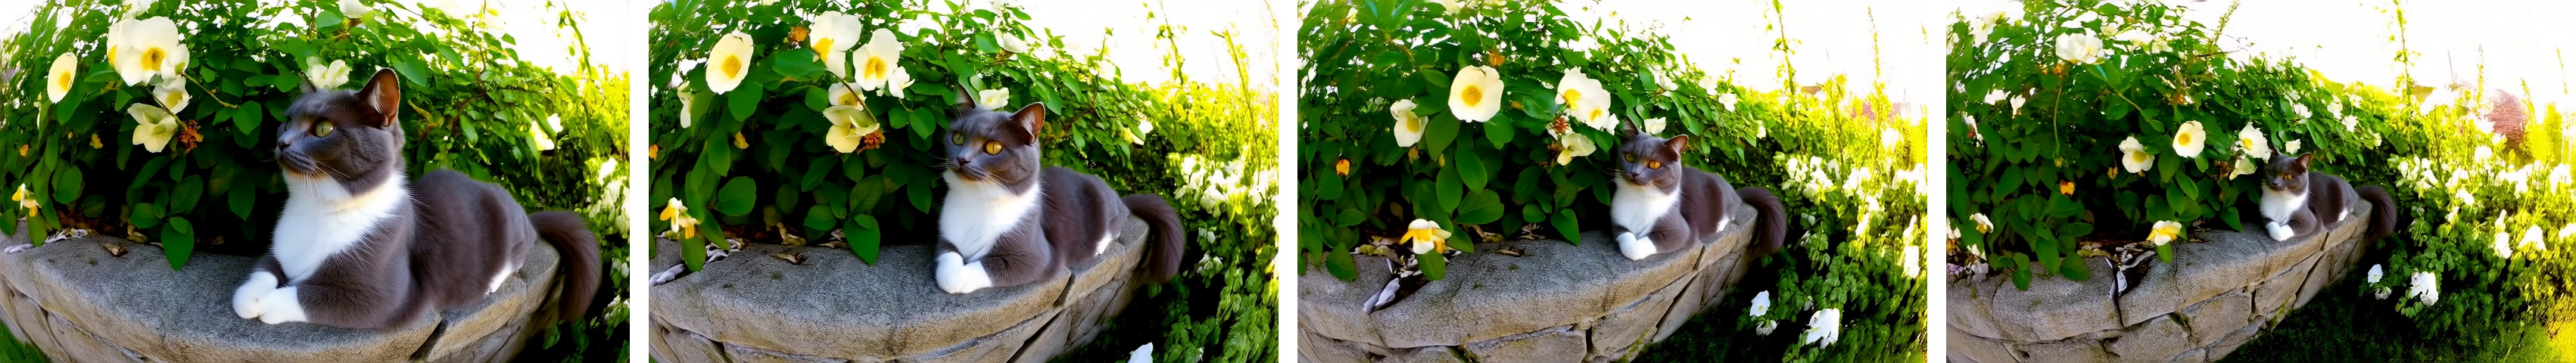
\includegraphics[width=1.0\columnwidth]{figure/rebuttal/0-f74139ac48f19b3c-fov180-xi2.00-A_flat,_telephoto_portrait_of_a_fluffy_gray_cat_lo-0.jpg}
    \caption{\textbf{Robustness to Text-Camera Conflict.} Even when the text prompt specifies a ``telephoto'' view, UCPE correctly synthesizes a fisheye video according to the provided camera parameters, resolving the conflict between text and geometry.}
    \label{fig:conflict}
\end{figure}

\paragraph{Generalization to Unseen Camera Models.}
UCPE is model-agnostic as it learns universal ray-space interactions.
For unobserved lens types, one can simply replace the ray-mapping function at inference to achieve control without fine-tuning, as the attention mechanism reasons about ray relationships rather than specific camera parameters (\eg, \(\xi\)).
We evaluate this capability on the complex Brown-Conrady camera model used in OpenCV for physical lens calibration (\(\textrm{xFoV} = 100^\circ, k_1 = -0.2, k_2 = -0.05\)).
As shown in \cref{fig:brown_conrady}, UCPE successfully generalizes to this model, adding realistic barrel distortion to the synthesized frames without requiring additional training.

\begin{figure}[t]
    \centering
    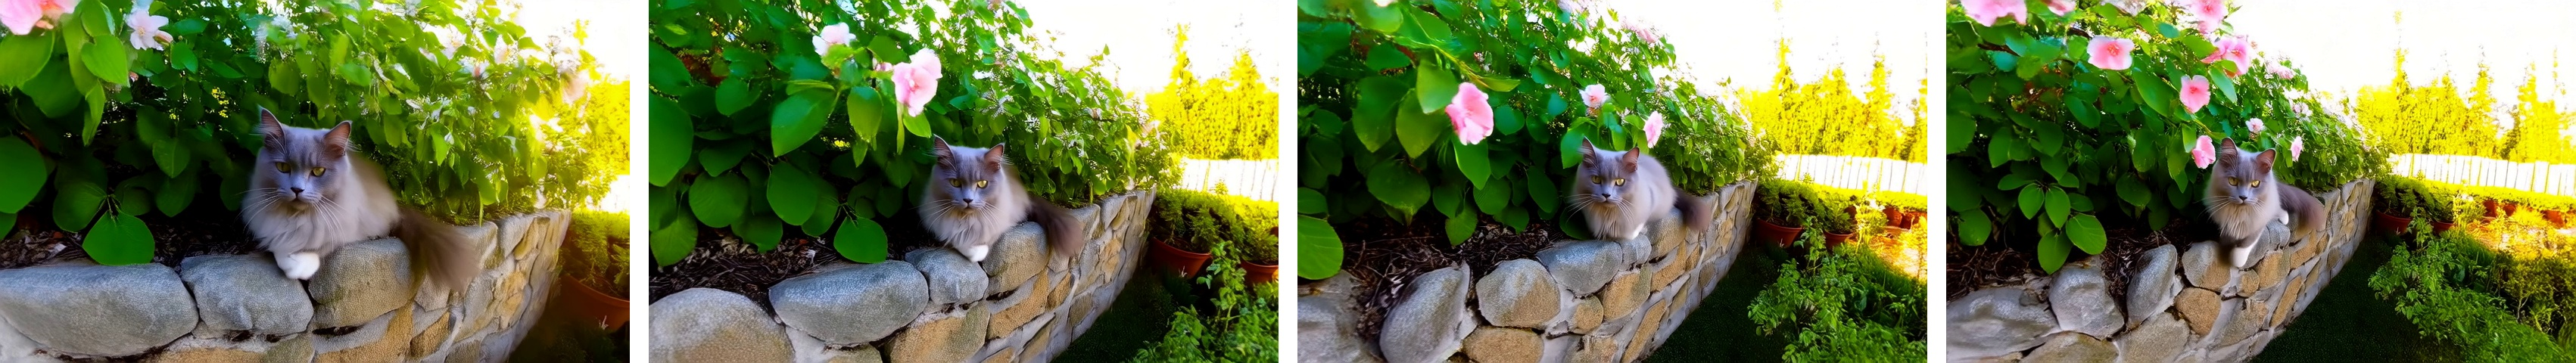
\includegraphics[width=1.0\columnwidth]{figure/rebuttal/0-f74139ac48f19b3c-fov100-k1-0.20-k2-0.05-A_fluffy_gray_cat_lounging_on_a_garden_stone_wall_-0.jpg}
    \caption{\textbf{Generalization to Unseen Camera Models.} Without fine-tuning, UCPE generalizes to unobserved models such as the Brown-Conrady model by simply substituting the ray-mapping function at inference time.}
    \label{fig:brown_conrady}
\end{figure}

\paragraph{Limitations.}
UCPE relies on camera poses during training and currently models only pose, intrinsics, and distortion, without capturing richer attributes such as zoom, focus, or depth-of-field.
Furthermore, we test UCPE with the ray-mapping function of Equirectangular projection (ERP), representing an extreme case not seen during training.
As shown in \cref{fig:failure_erp}, while UCPE fails to synthesize full 360° panoramas correctly under this extreme setting, we expect its performance to improve with targeted fine-tuning on panoramic datasets.

\begin{figure}[t]
    \centering
    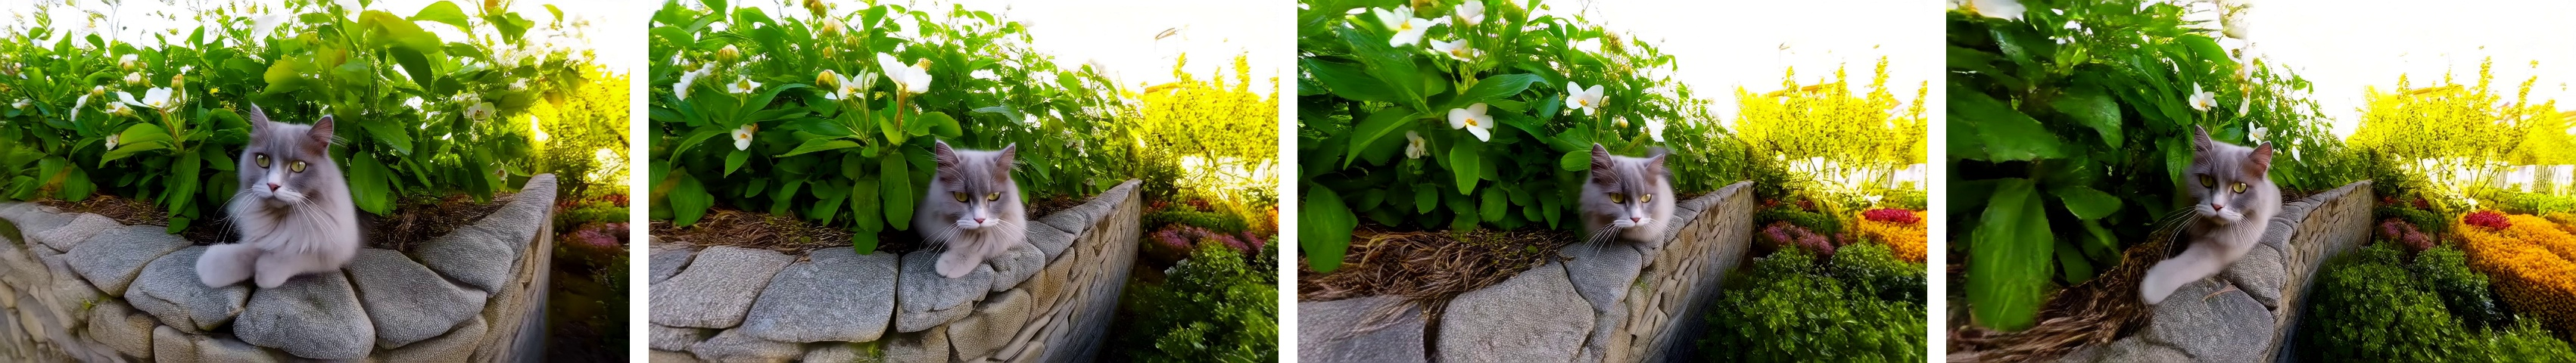
\includegraphics[width=1.0\columnwidth]{figure/rebuttal/0-f74139ac48f19b3c-ERP-A_fluffy_gray_cat_lounging_on_a_garden_stone_wall_-0.jpg}
    \caption{\textbf{Failure Case on Equirectangular Projection.} Testing with ERP ray-mapping results in artifacts as the model was not trained on such extreme panoramic projections.}
    \label{fig:failure_erp}
\end{figure}

\paragraph{Future Works.}
Extending UCPE to support these additional controls and further reducing reliance on accurate pose supervision (\eg, through self-supervised geometric losses) remain promising directions. 
Furthermore, while T2V generation is our primary focus, UCPE is also applicable to Image-to-Video (I2V) tasks. 
In contrast to T2V, I2V tasks benefit from the strong rigid pixel constraints of the input image, which naturally anchors the lens and initial orientation. 
Consequently, UCPE supports the I2V task without the need for Absolute Orientation Encoding (AOE): once the lens is defined (\eg, via GeoCalib), Relative Ray Encoding (RRE) alone can drive subsequent frames. 
To demonstrate this feasibility, we fine-tune Wan2.1-I2V-14B. 
As shown in~\cref{fig:supp_i2v}, our representations readily extend to control the camera pose in more constrained I2V settings. 
Video-to-Video (V2V) tasks (\eg, ReCamMaster) could similarly benefit from UCPE's enhanced controllability. 
Since such tasks inherently require synthetic multi-trajectory datasets, we leave this exploration to future work.


\begin{figure}[t]
    \centering
    \includegraphics[width=1.0\columnwidth]{figure/rebuttal/i2v.pdf}
    \caption{\textbf{Application to I2V Tasks.} We fine-tune Wan2.1-I2V-14B to demonstrate the feasibility of UCPE on more constrained Image-to-Video tasks.}
    \label{fig:supp_i2v}
\end{figure}




\section{Supplementary Video}
\label{sec:demo}

The supplementary video provides visualizations and demonstrations of the following aspects:
\begin{itemize}
    \item Overview of UCPE (Unified Camera Positional Encoding) and its two components: Relative Ray Encoding and Absolute Orientation Encoding.
    \item Demonstration of controllability over intrinsics and distortions.
    \item Demonstration of controllability over extrinsics and initial camera orientation.
    \item Applications enabled by UCPE, including cinematic content creation, autonomous driving, and embodied AI.
    \item Examples from our large-scale synthetic dataset with diverse intrinsics, distortion profiles, and camera motions (Sec.~4.1 of the main paper, Sec.~A of the supplementary).
    \item Comparison with baseline methods on our synthetic dataset for complete camera-controlled video generation (Fig.~4 of the main paper).
    \item Generalization results on the RealEstate10K dataset, showcasing improved camera controllability and video quality under pinhole camera settings (Fig.~5 of the main paper).
\end{itemize}





